

\documentclass[final]{beamer}

% ====================
% Packages
% ====================
\usepackage{amsfonts}
\usepackage[T1]{fontenc}
\usepackage{lmodern}
\usepackage[size=custom,width=120,height=72,scale=1.0]{beamerposter}
\geometry{paperwidth=42in,paperheight=32.5in}
\usetheme{gemini}
\usecolortheme{ucf}
\usepackage{graphicx}
\usepackage{booktabs}
\usepackage{tikz}
\usepackage{pgfplots}
\pgfplotsset{compat=1.17}

% ====================
% Lengths
% ====================

% If you have N columns, choose \sepwidth and \colwidth such that
% (N+1)*\sepwidth + N*\colwidth = \paperwidth
\newlength{\sepwidth}
\newlength{\colwidth}
\setlength{\sepwidth}{0.025\paperwidth}
\setlength{\colwidth}{0.3\paperwidth}

\newcommand{\separatorcolumn}{\begin{column}{\sepwidth}\end{column}}

% ====================
% Title
% ====================

\title{Facial Recognition Using Local Binary Pattern Histogram (LBPH) Algorithm}

\author{Anshul Malviya \inst{1} \and Prateek Daherwal \inst{2}\and Piyush Makde\inst{3}}

\institute[shortinst]{ \textit{Indian Institute of Information Technology, Nagpur} \samelineand}

% ====================
% Footer (optional)
% ====================

\footercontent{Submitted By: Anshul Malviya (CTGH21ECE601) | Prateek Daherwal (CTGH21ECE602) | Piyush Makde (CTGH21CSE406)\hfill
  Guided By: Dr. Tapan Jain}
% (can be left out to remove footer)

% ====================
% Logo (optional)
% ====================

% use this to include logos on the left and/or right side of the header:
% \logoright{\includegraphics[height=7cm]{logo1.pdf}}
% \logoleft{\includegraphics[height=7cm]{logo2.pdf}}

% ====================
% Body
% ====================

\begin{document}
\addtobeamertemplate{headline}{}
{
    \begin{tikzpicture}[remember picture,overlay]
      \node [anchor=north west, inner sep=3cm] at ([xshift=0.0cm,yshift=3cm]current page.north west)
      {
\includegraphics[height=8.5cm]{logos/lab_logo.png}}; % also try shield-white.eps

    \end{tikzpicture}
}

\begin{frame}[t]
\begin{columns}[t]
\separatorcolumn

\begin{column}{\colwidth}

  \begin{block}{Abstract}


The Local Binary Pattern Histogram (LBPH) algorithm is a face recognition algorithm based on a local binary operator, designed to recognize both the side and front face of a human. However, the recognition rate of the LBPH algorithm is limited, if the conditions, such as in the expression diversification, disorientation, and a change in the lighting performance manifest.

Local Binary Pattern (LBP) is a simple yet very efficient texture operator which labels the pixels of an image by thresholding the neighborhood of each pixel and considers the result as a binary number.

  \end{block}

  \begin{block}{Introduction}

Facial recognition is the ability to identify faces in an image, and then link them to a particular person. The LBPH is a recognition algorithm, which can recognize human faces.

It was first described in 1994 (LBP) and has since been found to be a powerful feature for texture classification. It has further been determined that when LBP is combined with histograms of oriented gradients (HOG) descriptor, it improves the detection performance considerably on some datasets.

Face recognition can be achieved with the help of a learning concept of training and then testing the model with a given set of images.

Training rules are used to ensure the output decisions criteria and training algorithm can be used to get some input from the data to match the appropriate output type. So, the algorithm and rules are used to simplify the process of learning. The system uses the information gathered from the data to get results.


  \end{block}
  \begin{block}{Working of the LBPH Algorithm}

\heading{The LBPH algorithm typically makes use of 4 parameters:}

Radius: The distance of the circular local binary pattern from the center pixel to its circumference and usually takes a value of 1.

Neighbors: The number of data points within a circular local binary pattern. Usually, the value of 8.

Grid X: The number of cells in the horizontal plane, is usually a value of 8.

Grid Y: The number of cells in the vertical plane, is usually a value of 8.

Given the above-mentioned parameters, LBPH works as follows,

A data set is created by taking images with a camera or taking images that are saved, and then provisioning a unique identifier or name of the person in the image and then adding the images to a database. It is recommended to take many samples from a single individual. A portion of the data set is used for the training of the algorithm, while the rest is used for testing.

Using a circular neighborhood concept (which takes non-integer pixel points around a selected area), the number of appearances of LBP codes in the image is put together to form a histogram. The classification is then carried out through the calculation of the basic similarities of the histograms under comparison.



  \end{block}

\end{column}

\separatorcolumn

\begin{column}{\colwidth}

  \begin{block}{Two modes of operation of face recognition}

\heading{The two modes of operation of face recognition is,}

{1. Authentication of a facial image} \newline
{2. Face recognition} 


Authentication of a facial image: This mode does facial recognition by a 1x1 comparison. The comparison is done between an input image and a specific image within the database. In many cases, this is the face that requires authentication at the time of this mode of facial recognition.

Face recognition: in this mode, it is a 1xN, a comparison of the input face image with all the pictures that have been saved in the database to output the images of the user which conforms to the input face image.





  \end{block}

\graphicspath{ {./logos} }
  \begin{block}{The stages of face recognition using LBPH}
  
 \heading{For face recognition, the LBPH algorithm follows some steps. These steps can be carried out in two stages, as follows:}

The first step is the learning of the algorithm. It makes use of a data-set of images of the people to be included in the recognition process. Each image is given a unique ID as either a number or the name of a person so that the algorithm can use this information to identify the image and export the output. The pictures of the same person are always placed under the Computational steps

The application of the LBP operation: is the first step of the computational steps. Here, an intermediate image has been created to better represent the original image through a sliding window concept, taking into account two parameters: the neighbor and the radius. New values are created in the form of binary by comparing the 8 neighbor values to the threshold value. For each neighbor value greater than the threshold value, the value is set to 1 and 0 for every neighbor value less than the threshold value. This forms a matrix of binary numbers excluding the threshold. A central value of the matrix is created by the conversion of the binary number to a decimal value which corresponds to the pixels of the original image. For a better representation of the characteristics of the original.

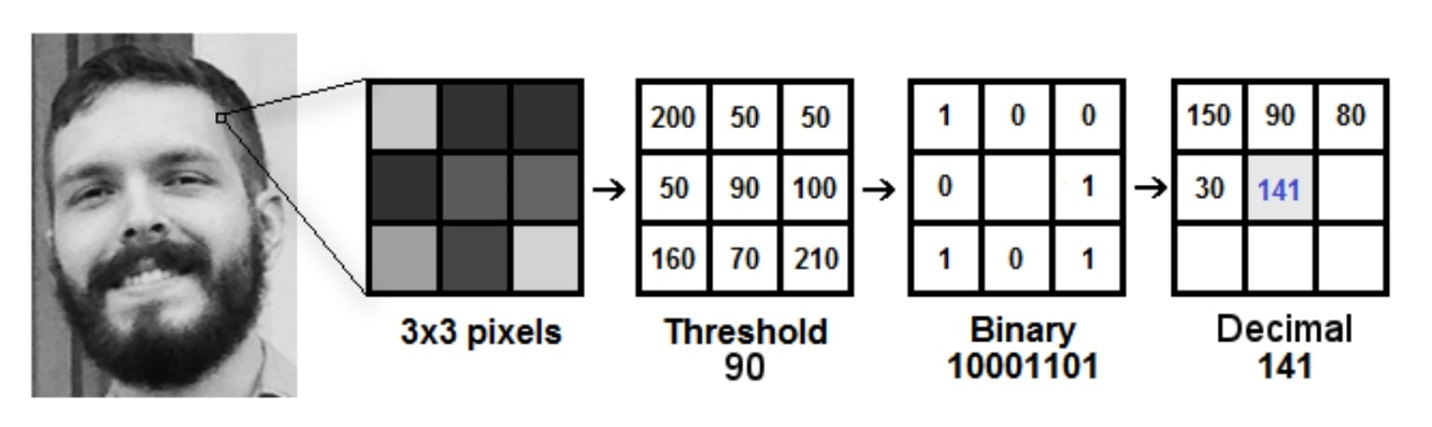
\includegraphics{figure11}

\begin{center}
    \caption{Figure 1. Image to Binary Pattern}  \hfill
\end{center}

To Extract Histograms: The image obtained in step is divided into multiple grids, with the help of the Grid parameters X and Y. This image is in grayscale, each of the histograms of each of the grids is to represent the intensity of the occurrences of each pixel. Each histogram is then combined to create a new histogram that represents the attributes of the original image.
 

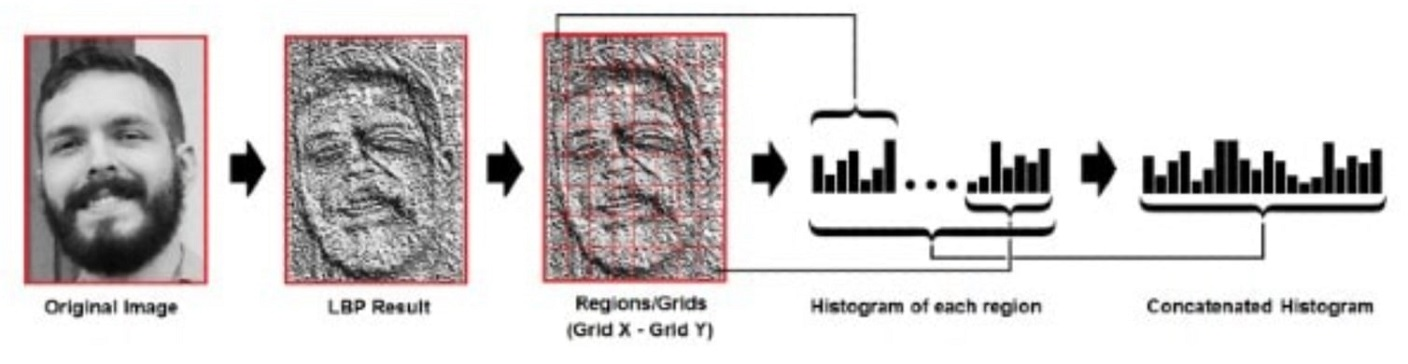
\includegraphics{figure21}
\begin{center}
    \caption{Figure 2. Binary Pattern to Histogram}  
\end{center}


Accurate face recognition: Each one made a histogram for an image in the training data set. Two histograms are compared to output the image with the closest histogram matches to an input image.


  \end{block}

  
    
   

 

\end{column}

\separatorcolumn

\begin{column}{\colwidth}

  \begin{block}{Applications}

Texture analysis: applicable in research and in applications such as medical imaging. This has made image processing easy due to texture segmentation of images which has led to a significant progress in analysis.

Biometrics: used in biometrics, such as palm-print recognition, fingerprint recognition, iris recognition, gait recognition, the order of placement of recognition, and in the face of an age rating.

Computer vision: used in computer vision such as motion analysis. LPH enables computer systems to be able to understand information on images and make meaning of this information.


  \end{block}

  \begin{block}{Conclusion}

1. LBPH is one of the easiest face recognition algorithms.

2. It can represent local features in the images.

3. It is possible to get great results (mainly in a controlled environment).

4. It is robust against monotonic grey scale transformations.

5. It is provided by the OpenCV library (Open Source Computer Vision Library).

  \end{block}

  \begin{block}{References}

https://www.analyticsvidhya.com/blog/2021/07/understanding-face recognition-using-lbph-algorithm/

https://towardsdatascience.com/face-recognition-how-lbph-works-90ec258c3d6b

https://pyimagesearch.com/2021/05/03/face-recognition-with-local-binary-patterns-lbps-and-opencv/

https://iq.opengenus.org/lbph-algorithm-for-face-recognition/



  \end{block}
  \graphicspath{ {./logos} }
  \begin{block}{QR Code for Repository}
\newline
\newline


  \centering
    
\includegraphics[width=0.50\textwidth]{logos/LBPH QR.png}


  \end{block}

\end{column}

\separatorcolumn
\end{columns}
\end{frame}

\end{document}
